% -----------------------------------------------------------------------------
% Master thesis in the study program computational mechanics
%
% B.Sc. Rezha Adrian Tanuharja - 03751261
% M.Sc. Felix Schneider (supervisor)
%
% chapters/discussion/substructuring/point_A.tex
% Last edited 03 November 2023
% -----------------------------------------------------------------------------

\subsection{Vertical Acceleration at Node A}
\label{ssec: cms point A}

Figure \ref{FRF_MC_A_A_linear} shows the FRFs from direct MCS of the complete plate model.
These FRFs relate the vertical acceleration magnitude at point A to a unit force at the same point at discrete frequencies in the range $\left[9.0, 17.5\right]$ rad/s with increments of $0.5$ rad/s.
The outliers are intentionally missing to enable a clear view of the FRFs' statistics: their medians, interquartile ranges, and whiskers.
\begin{figure}[H]
    \centering
    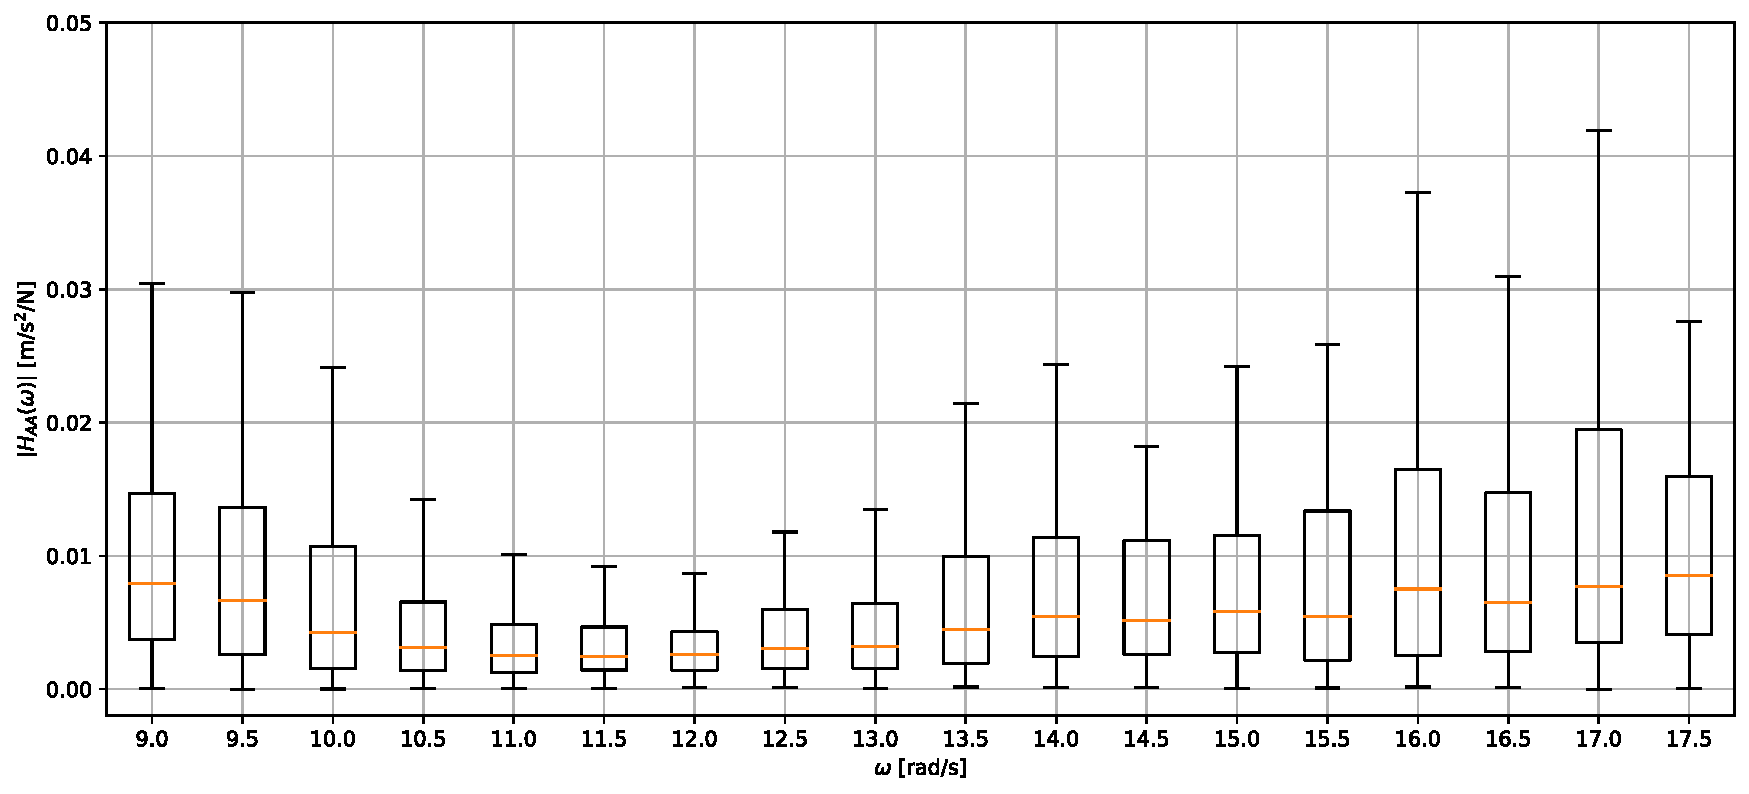
\includegraphics[width=1.0\textwidth]{
        plots/substructuring/plot_1_linear.pdf
    }
    \caption{%
        $\left|H_{AA}\right|$ from Direct MCS of The Complete Plate Model
    }
    \label{FRF_MC_A_A_linear}
\end{figure}
Figure \ref{FRF_MC_A_A_log} shows the same FRFs as figure \ref{FRF_MC_A_A_linear} with outliers.
The logarithmic scale provides a clear view of the outliers and the low whiskers of the plot.
The figure shows that the outlier values can be larger by approximately two orders of magnitudes compared to the medians.
\begin{figure}[H]
    \centering
    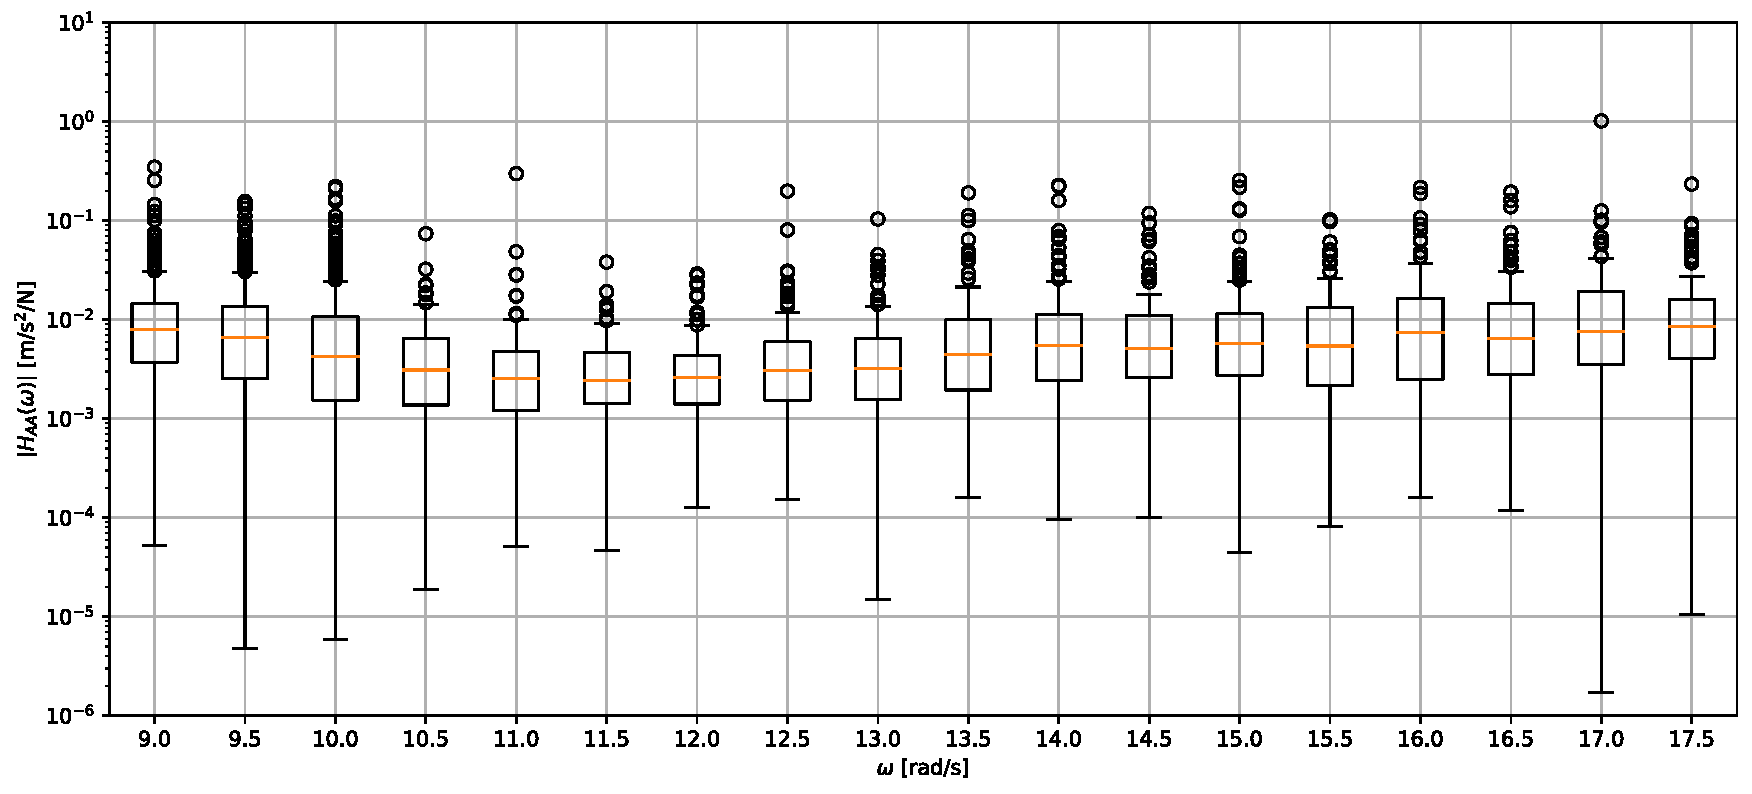
\includegraphics[width=1.0\textwidth]{
        plots/substructuring/plot_1_log.pdf
    }
    \caption{%
        $\left|H_{AA}\right|$ from Direct MCS of The Complete Plate Model with Outliers
    }
    \label{FRF_MC_A_A_log}
\end{figure}
First, the author analyzes the performance of the CUCB method.
Figure \ref{e_emp CUCB_A_A} shows the median relative empirical errors for the method in each frequency in the above range using three different numbers of internal modes.
The medians come from the bootstrapping method with a $1000$ number of resamplings.
\begin{figure}[H]
    \centering
    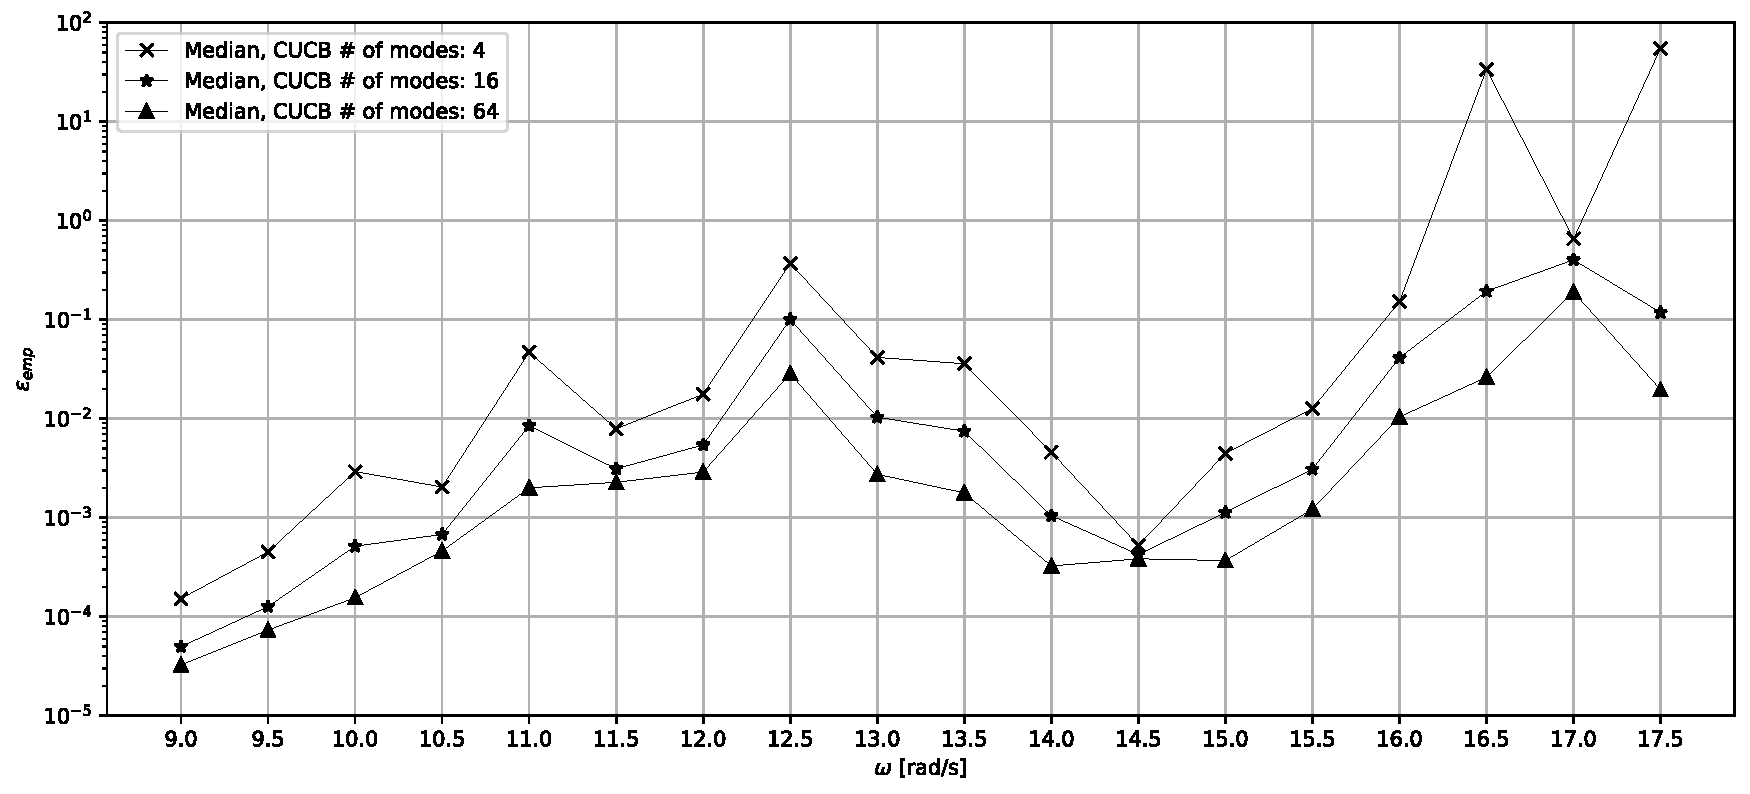
\includegraphics[width=1.0\textwidth]{
        plots/substructuring/plot_2.pdf
    }
    \caption{%
        Relative Empirical Errors of $H_{AA}$ for The CUCB Method
    }
    \label{e_emp CUCB_A_A}
\end{figure}
In deterministic dynamic substructuring, errors decrease as the number of internal modes increases.
When all internal modes are present in the model, the assembled components are equivalent to the complete structure in a mathematical sense.
Figure \ref{e_emp CUCB_A_A} exhibits the same trend for dynamic structuring using the CUCB method: as the number of internal modes increases, the relative empirical errors decrease.
However, the relative empirical errors exceeds $10^{-1}$ at $\omega=17.0$ rad/s even when using $64$ internal modes.
Therefore, the mean square errors are in the same order of magnitude as the FRFs' variance at this frequency.

Subsequently, the author analyzes the performance of the HUCB method.
Figure \ref{e_emp HUCB_A_A} shows the medians and $95\%$ confidence intervals of the relative empirical errors for the crude and hybrid UCB methods.
Figure \ref{e_emp HUCB_A_A} shows that the relative empirical errors from the HUCB method do not exceed $10^{-2}$ in this example and in most frequencies in the range lie below $10^{-3}$.
The computational cost of the HUCB method is higher than that of the CUCB method because of the evaluation of the boundary modes for each input parameter's realization.
However, it leads to lower overall relative empirical errors and, in some frequencies, reduces the errors by up to two orders of magnitudes.
\begin{figure}[H]
    \centering
    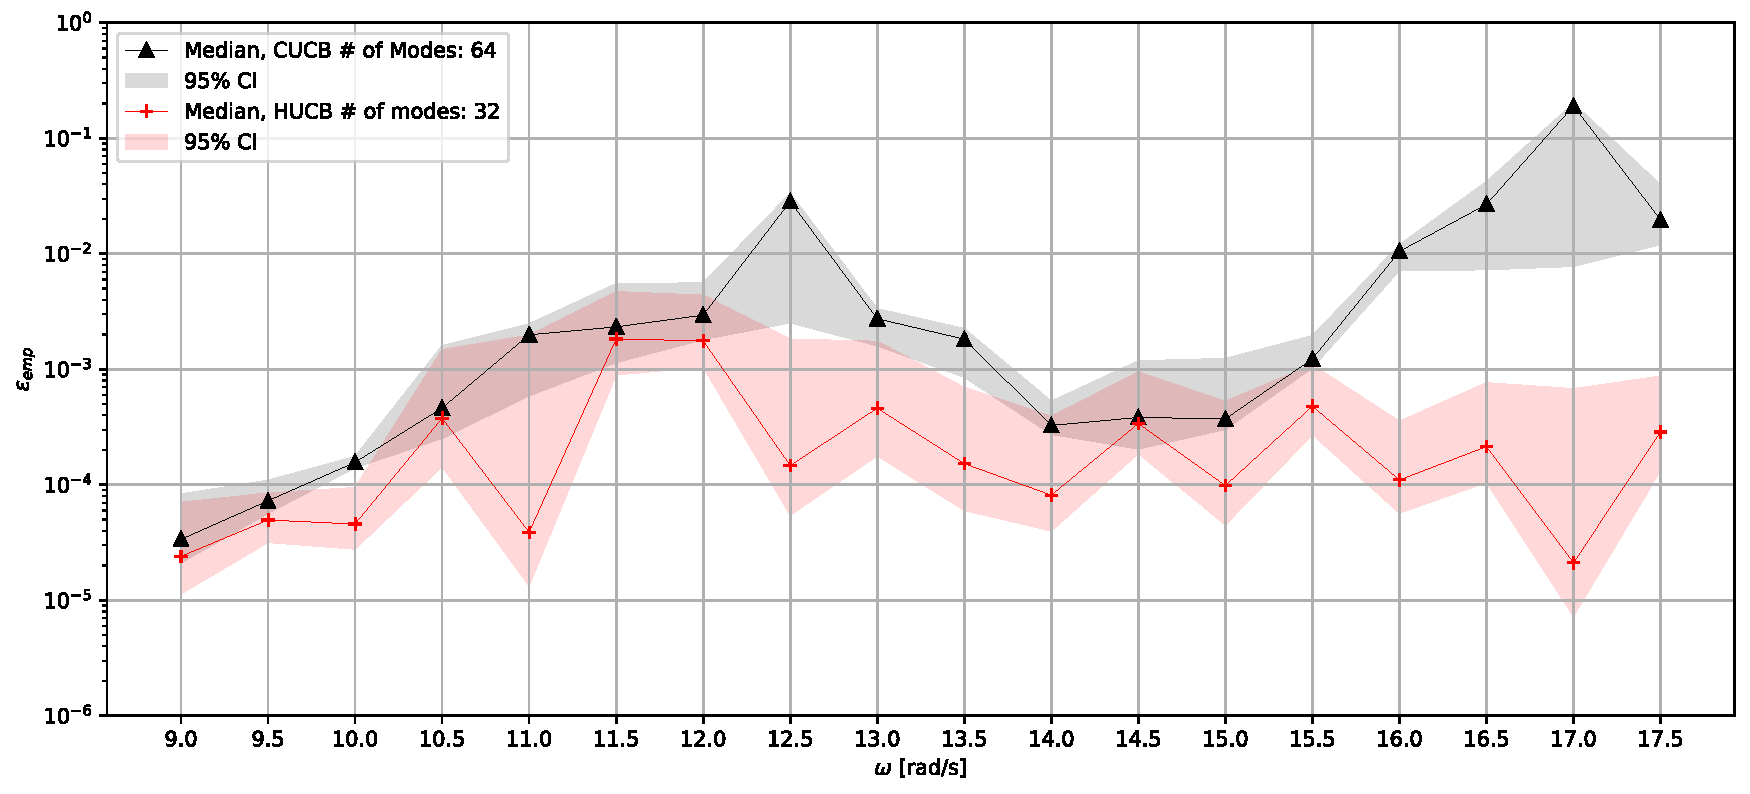
\includegraphics[width=1.0\textwidth]{
        plots/substructuring/plot_3.pdf
    }
    \caption{%
        Relative Empirical Errors of $H_{AA}$ for The CUCB and HUCB Methods
    }
    \label{e_emp HUCB_A_A}
\end{figure}

To dive deeper into the difference between the crude and hybrid UCB methods, the author evaluates the relative mean and variance errors.
Figure \ref{e_mean CUCB_A_A} shows the median relative mean errors of the FRFs' magnitudes for the CUCB method using three different numbers of internal modes.
\begin{figure}[H]
    \centering
    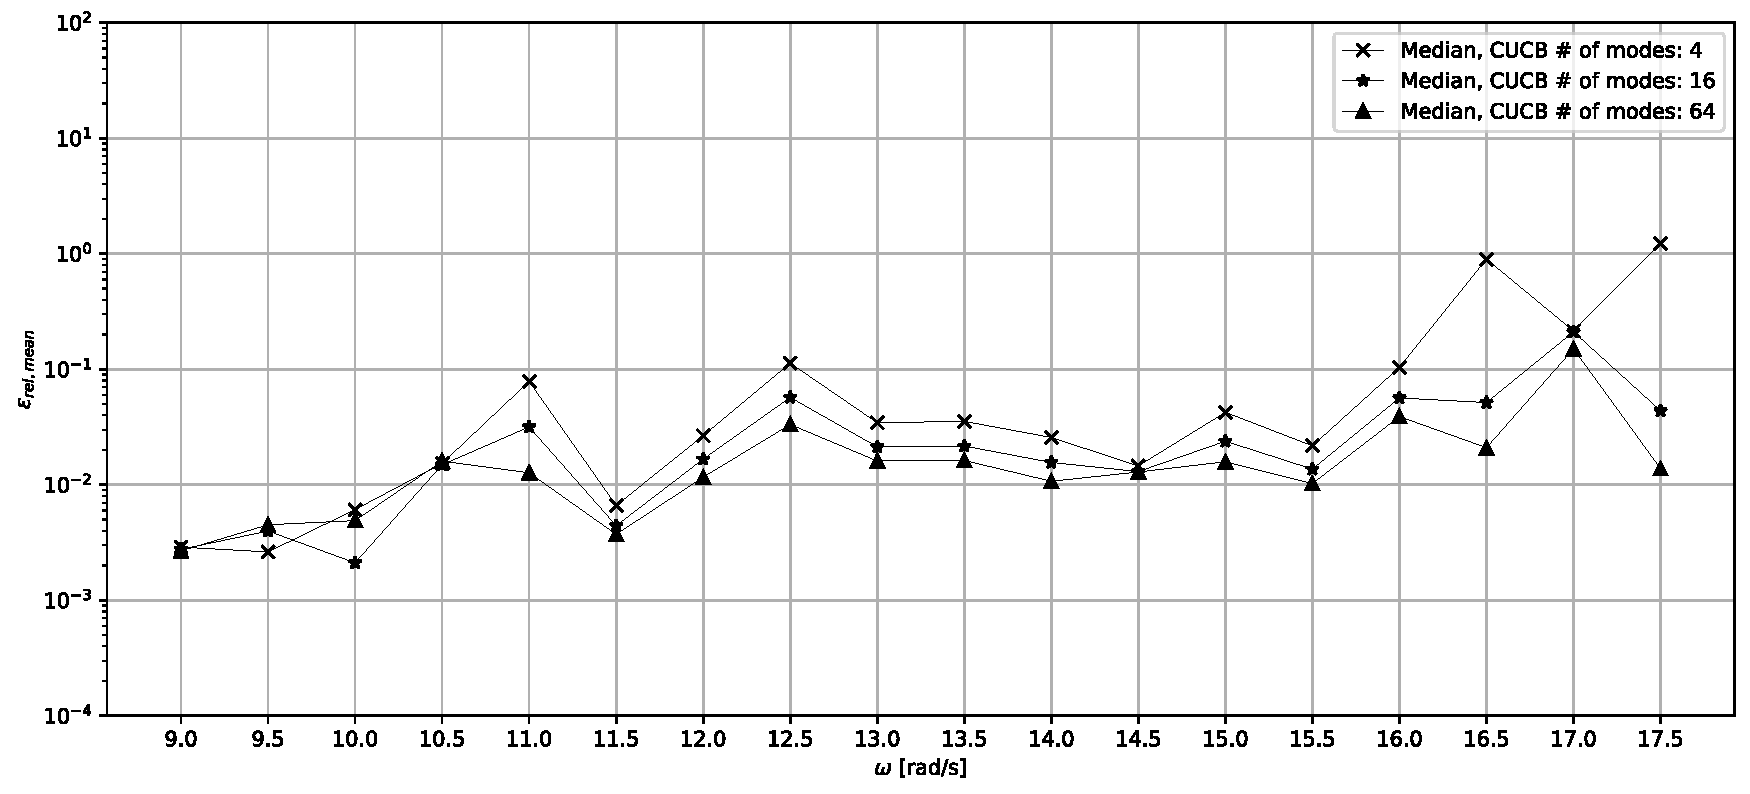
\includegraphics[width=1.0\textwidth]{
        plots/substructuring/plot_4.pdf
    }
    \caption{%
        Relative Mean Errors of $\left|H_{AA}\right|$ for The CUCB Method
    }
    \label{e_mean CUCB_A_A}
\end{figure}
Figure \ref{e_var CUCB_A_A} shows the median relative variance errors of the FRFs for the CUCB method using three different numbers of internal modes.
\begin{figure}[H]
    \centering
    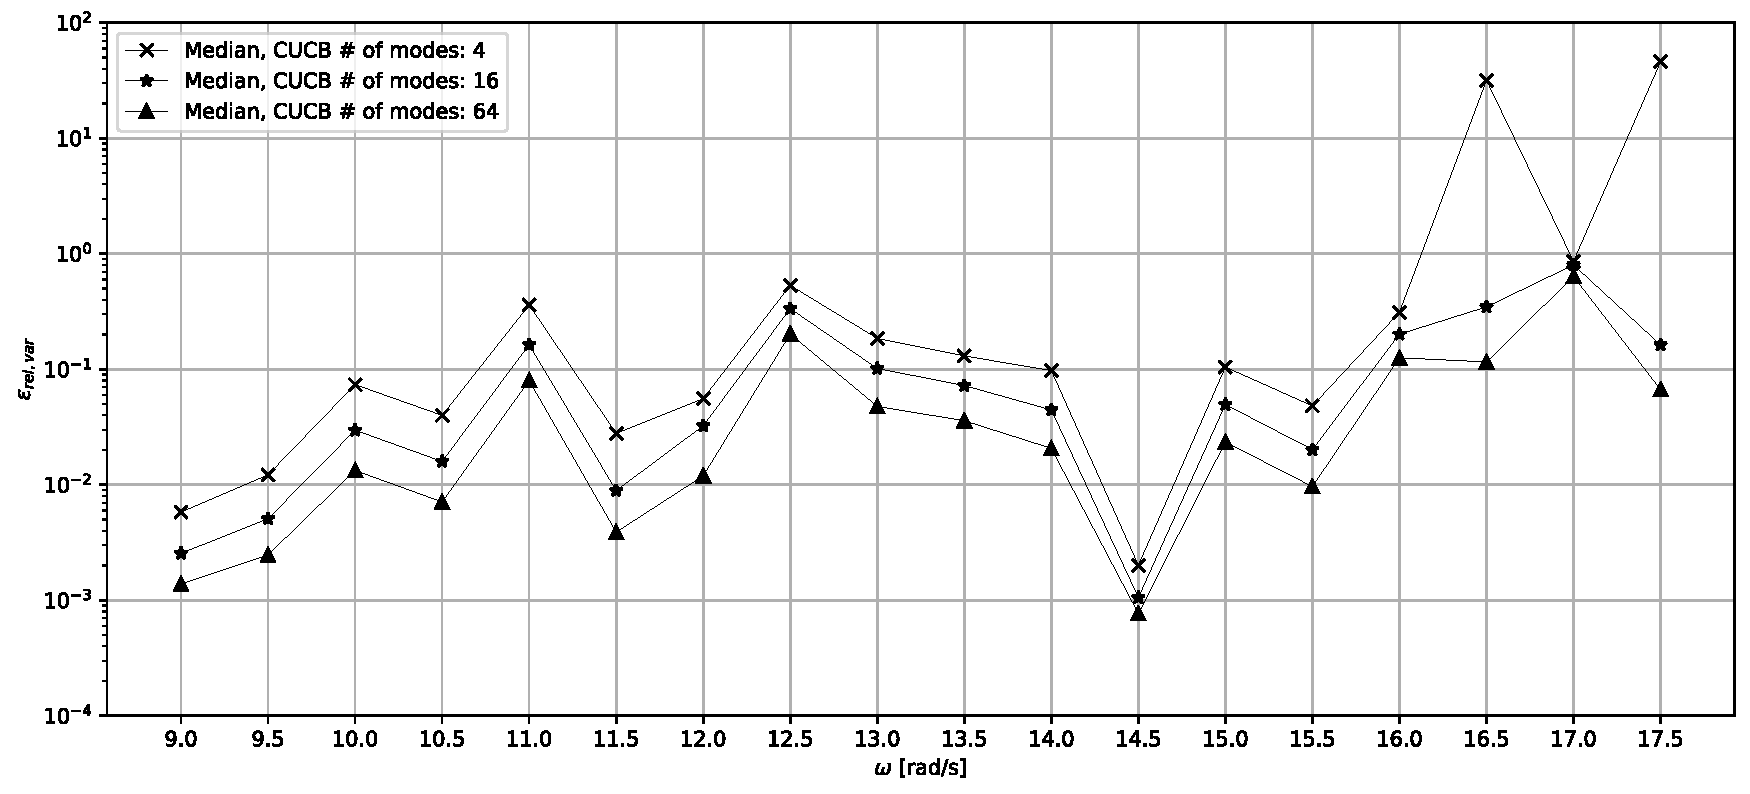
\includegraphics[width=1.0\textwidth]{
        plots/substructuring/plot_5.pdf
    }
    \caption{%
        Relative Variance Errors of $H_{AA}$ for The CUCB Method
    }
    \label{e_var CUCB_A_A}
\end{figure}
The two figures above exhibit similar trends with figure \ref{e_emp CUCB_A_A}: the relative mean errors decrease as the number of internal modes increases, with an exception at $\omega=9.5$ rad/s for the relative mean errors.
Overall, the relative mean errors and relative variance errors primarily lie between $10^{-3}$ and $10^{0}$.

Subsequently, the author compares the relative mean errors and relative variance errors for the CUCB method and the HUCB method.
Figure \ref{e_mean HUCB_A_A} shows the medians and $95\%$ confidence intervals of the relative mean errors of the FRFs' magnitudes in each frequency in the above range for the crude and hybrid UCB methods.
\begin{figure}[H]
    \centering
    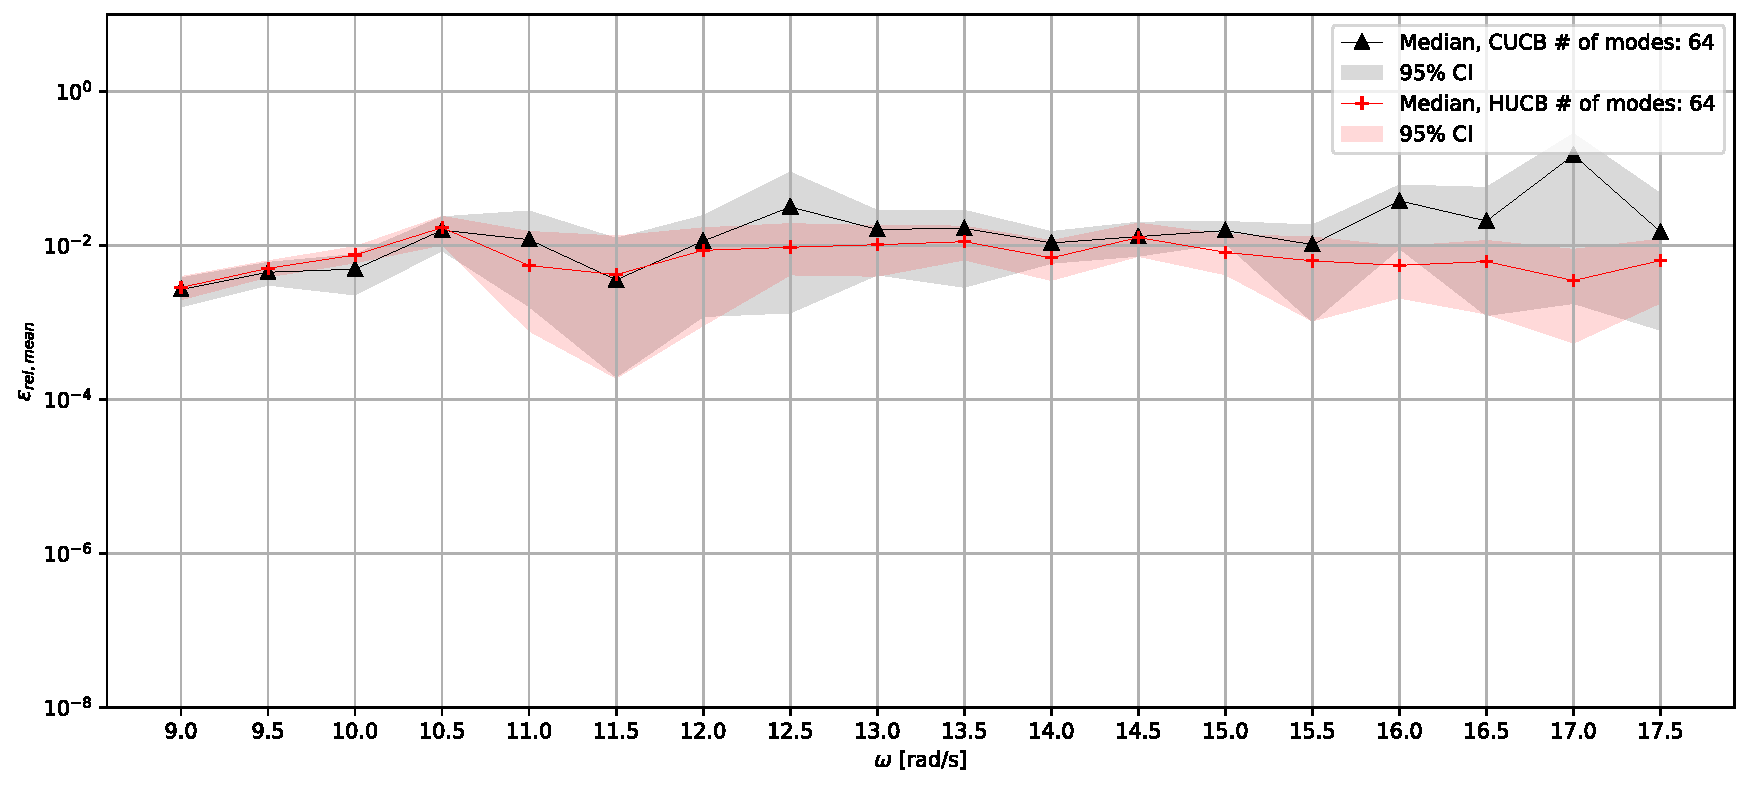
\includegraphics[width=1.0\textwidth]{
        plots/substructuring/plot_6.pdf
    }
    \caption{%
        Relative Mean Errors of $\left|H_{AA}\right|$ for The CUCB and HUCB Methods
    }
    \label{e_mean HUCB_A_A}
\end{figure}
Figure \ref{e_var HUCB_A_A} shows the median and $95\%$ confidence interval of the relative variance error for the FRFs' magnitudes in each frequency in the above range using the crude and hybrid UCB methods.
\begin{figure}[H]
    \centering
    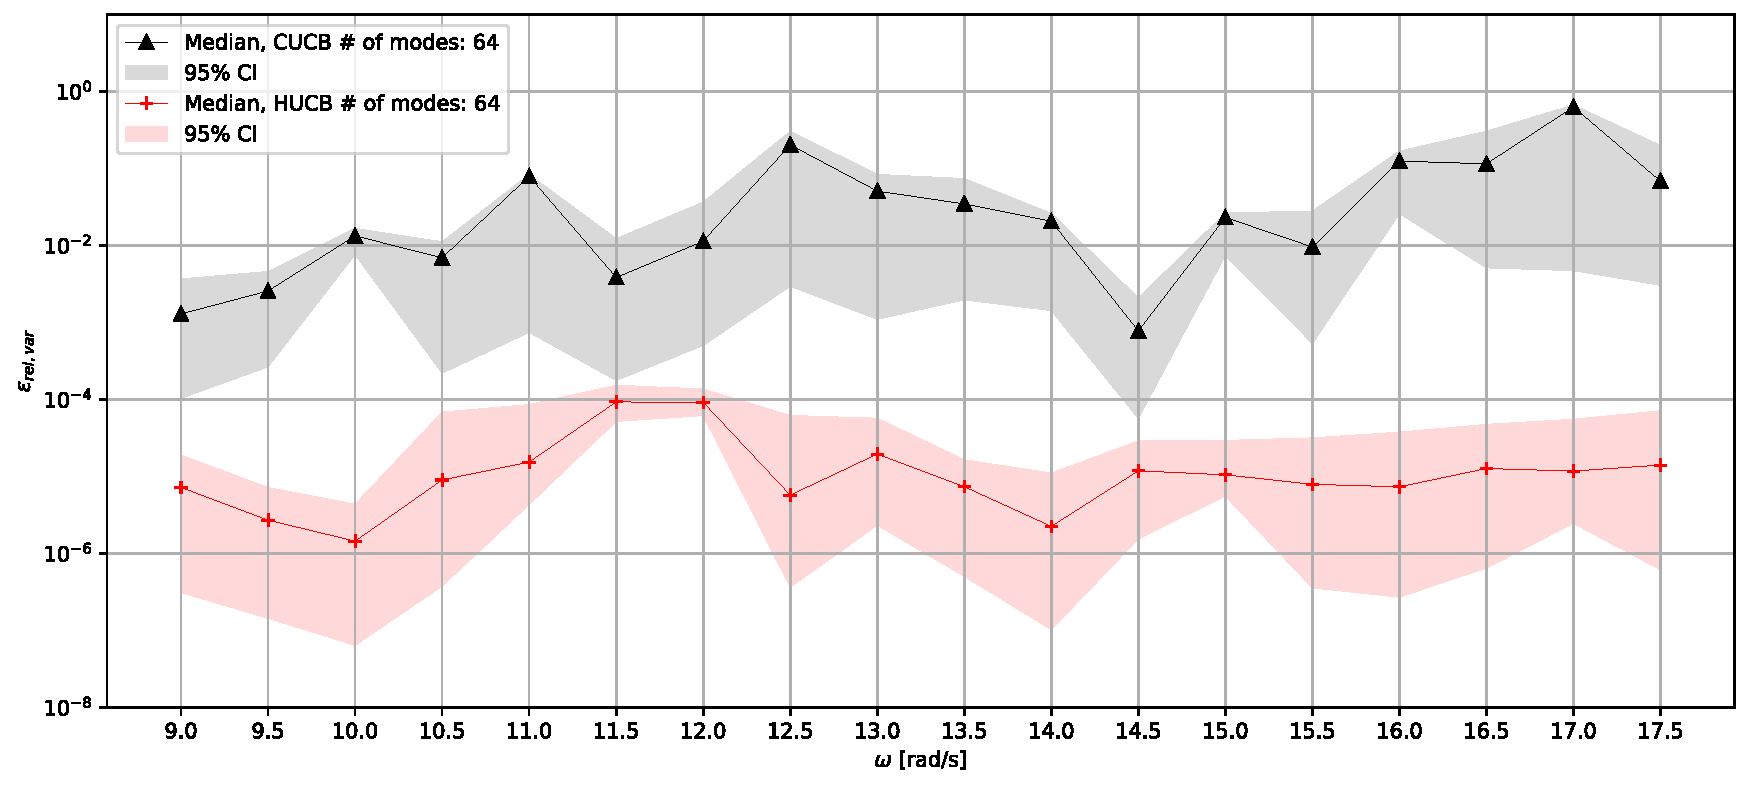
\includegraphics[width=1.0\textwidth]{
        plots/substructuring/plot_7.pdf
    }
    \caption{%
        Relative Variance Errors of $H_{AA}$ for The CUCB and HUCB Methods
    }
    \label{e_var HUCB_A_A}
\end{figure}
The two figures above show that while the relative mean errors from the two approaches are comparable, the HUCB method better approximates the FRFs' variabilities, thus leading to lower overall relative empirical error.